\documentclass[10pt,a4paper, nocenter]{report}
\usepackage[scaled=0.92]{helvet}
\usepackage[margin=1in]{geometry}
\usepackage[latin1]{inputenc}
\usepackage{blindtext}
\usepackage{amsmath}
\usepackage{appendix}
\usepackage{amsfonts}
\usepackage{amssymb,amsthm}
\usepackage{graphicx}
\usepackage{parskip}
\usepackage{fancyhdr}
\usepackage{lastpage}
\usepackage{enumerate,url}
\usepackage{etoolbox}
\usepackage{algorithm2e}
\makeatletter
\patchcmd{\chapter}{\if@openright\cleardoublepage\else\clearpage\fi}{}{}{}
\makeatother
\makeatletter
\patchcmd{\chapter}{\@maketitle\cleardoublepage}{}{}{}
\makeatother

\newtheorem{prop}{Proposition}
\newtheorem{theorem}{Theorem}
\newcommand{\abs}[1]{\lvert {#1} \rvert}
\newcommand{\norm}[1]{\lvert\lvert {#1} \rvert\rvert}


\pagestyle{fancy}
\lhead{[WORK IN PROGRESS] \\ Research Report - Spectral Clustering}
\rhead{Sourabh Antani}
\cfoot{\thepage\ of \pageref{LastPage}}
\renewcommand{\footrulewidth}{0.4pt}


\author{Sourabh Antani}
\title{[WORK IN PROGRESS] \\ Research Report - Spectral Clustering}
\date{}

\begin{document}
	\maketitle

	
	\chapter{Introduction}
    \thispagestyle{fancy}
    Now a days, Clustering has become one of the most fundamental tasks in any project involving exploratory data analysis. Clustering helps the researchers understand the diversity of the data and number of different populations that exist. This knowledge, in turn, aids in subsequent tasks like choice modelling or classification techniques or parameters for tuning them. 
	
    In this report, I will list some of the commonly used clustering techniques before diving deeper into Spectral Clustring. Thereafter we will look at some of the common challanges with spectral clustering and some of the existing advancements that have been proposed to alleviate them. Finally I will list some of the possible avenues of research that I wish to research. 

    \section*{Clustering Algorithms}
    In practice, apart from Spectral Clustering, various types of clustering algorighms are used, ranging from the ones based on spatial distribution to matrix factorization to eigen-value based methods. 
    
    Some common examples of algorighms that rely on euclidean distance and spacial density of points are $k$-means (term first used by J. Macqueen \cite{Macqueen67kmeans}, standard algorithm published by Lloyd \cite{Lloyd-82-kmeans}), which iteratively computes the controids of the clusters using euclidean distances, BIRCH (Balanced Iterative Reducing and Clustering using Hierarchies)\cite{zhang-96-birch}, which extracts centroids from building Hierarchies, mean-shift\cite{Cheng95meanshift} and DBSCAN \cite{Ester96adensity-based}, which locates the centroids by iteratively following the higher density areas. while these are generally simpler to understand, the 'shape' of the spatial distribution greately affects the effectivenes of these algorithms. 

    Non-Negative Matrix Factorization \cite{Lawton-1971-nnmf} \cite{Paatero1991-nnmf} (later \cite{Ding05-nnmf-spectral} studied the equivalence of NNMF with Spectral Clustering) and PCA Based clustering \cite{Zhang-2108-pca} are examples of techniques based on matrix factorization. These techniques seek to factorize the matrix and use one of the factors as approximate basis for the matrix, thus effectively reducing the dimentionality of the problem. Another advantage of these methods is that it simple to guage how 'good' the approximation is by looking at the difference between the product of approximated factors and the original matrix. Thus finding out the number of 'extracted' features or reduced dimention that captures the desired variability in the data. 


    \chapter{Spectral Clustering}
    An excellent tutorial to Spectral Clustering can be found in \cite{Luxburg2007}. Before we look at the various algorithms, let us go through some basic terms involved.

    \section{Some Terminology}

        Given an undirected graph $G=(V,E)$ with $V=\{v_{1},\dots,v_{n}\}$ being the set of vertices and $E$ being the set of weighted edges such that each edge between two vertices $v_{i}$ and $v_{j}$ carries a non-negative weight $w_{ij} \ge 0$.

        The Weighted \textit{adjacency matrix} of the graph is the matrix $W=(w_{ij})_{i,j=1,\dots,n}$. If $w_{ij}=0$, vertices $v_{i}$ and $v_{j}$ are not connected. $w_{ij}=w_{ji}$ since $G$ is undirected. 

        The degree of a vertex $v_{i}\in V$ is defined as $ d_{i} = \sum_{j=1}^{n}w_{ij}$. \textit{degree matrix} $D$ is defined as the diagonal matrix with the degrees $d_{1} ,\dots, d_{n}$ on the diagonal. 

        $\bar{A}$ denotes the Complement $V \backslash A$  of a given subset $A \subset V$. Indicator vector $\mathbf{1}_{A}$ is a vector with entries $f_{i} = 1$ if $v_{i}=A$, $f_{i}=0$ otherwise.

        Define $W(A,B) = \sum_{i\in A, j\in B}w_{ij}$:], for not necessarily disjoint sets $A, B \subset V$.
        The 'size' of $A \subset V$ can be measured in two ways, $\lvert A \rvert$ := number of vertices in $A$ or $vol(A)$ := $\sum_{i\in A}d_{i}$

        A subset $A \subset V$ of a graph is connected if any two vertices in $A$ can be joined by a path such that all intermediate points also line in $A$. $A$ is called Connected Component if it is a connected subset such that $A$ and $\bar{A}$ are disjoint. FInally, Partitions of a graph are defined as non-empty sets $A_{1},\dots,A_{k}$ form partition of graph inf $A_{i} \cap A_{j} = \emptyset$ and $A_{1}\cup \dots \cup A_{k} = V$

    \section{Graph Laplacians and Graph cuts}

        The following types of graph Laplacians have been defined in the literature:
        \begin{align*}
         \textbf{Unnormalized Graph Laplacian: } &L = D- W \\
         \textbf{Normalized Graph Laplacian (Symmetric): } &L_{sym} = D^{-1/2}LD^{-1/2} = I - D^{-1/2}WD^{-1/2} \\
         \textbf{Unnormalized Graph Laplacian (Raondom walk): } &L = D^{-1}L = I - D^{-1}W 
        \end{align*}

        All three graph Laplacians are positive-semidifinte and have non-negative real valued eigen values. Also, 0 is an eigenvalue with multiplicity equal to number of connected components of the graph. Thus for fully connected graph one of the eigenvalues is 0. $L$ and $L_{sym}$ are symmetric. The eigenvectors of $L_{rw}$ are the eigen vectors of $L$ while $D^{1/2}u$ is eigenvector of $L_{sym}$ if $u$ is eigenvector of $L$. For proofs of the above properties, refer to the appendix. For information about unnormalized graph Laplacian, refer \cite{mohar-1991} and \cite{mohar-1997} while the standard reference for normalized graph Laplacian is \cite{graph-spectral-book}

        The intuition of clustering is to divide the graph in to groups of vertices such that he edges between the vertices in the same group have high weight and the edges between vertices from different groups have zero or very low weight. Thus effective clustering is to solve the minicut problem which can be defined as, for a given number $k$ subsets, choosing the a partition $A_{1}, \dots, A_{k}$ which minimizes $$ \text{cut}(A_{1}, \dots, A_{k}) := \frac{1}{2}\sum_{i-1}^{k}W(A_i,\bar{A}_{i}) $$

        In order to make sure that minicut does not simply spearate an individual vertex, two approaches have been suggested to make sure that the clusters are 'reasonably large'. 

        First is RatioCut \cite{hagen-kahng-1992} where the solution is to solve minicut problem while dividing the graph in components with roughly the same number of vertices. The second approach is Ncut \cite{Shi-Malik-maxcut-00} which tries to solve the minicut problem by keeping the volume of each component, i.e. sum of edge weights, roughly the same.
        
        Thus, the objective functions that we seek to minimize are
        \begin{align*}
            RatioCut(A_{1},\dots,A_{k}) &= \frac{1}{2} \sum_{i=1}^{k}\frac{W(A_{i},\bar{A}_{i})}{\lvert A_{i} \rvert}
            = \sum_{i=1}^{k}\frac{cut(A_{i},\bar{A}_{i})}{\lvert A_{i} \rvert} \\
            Ncut(A_{1},\dots,A_{k}) &= \frac{1}{2}\sum_{i=1}^{k}\frac{W(A_{i},\bar{A}_{i})}{vol(A_{i})} = 
            \sum_{i=1}^{k}\frac{cut(A_{i},\bar{A}_{i})}{vol(A_{i})}
        \end{align*}
    
        While the introduction of these balancing condition makes the mincut problem NP hard, relaxing these conditions slightly leads Ncut and RatioCut to normalized and unnormalized spectral clustering respectively \cite{Luxburg2007}

    \section{Algorithms}

    Three classic spectral clustering algorithms can be found in literature.

    All three algorithms essentially follow the same steps, using the first $k$ eigen vectors of the graph Laplacian, create a matrix and then create $k$ clusters from the rows of that matrix using k-Means algorithm. Finally, create the clusters of data points with the same indices as the indices of the matrix rows in the $k$ clusters formed by k-means. For a proof of how the relaxation of the above balancing conditions to arrive at an approximation of NCut and RatioCut leads to the Normalized and Unnormalized Spectral Clustering respectively, see \cite{Luxburg2007}
	
	\subsection{Unnormalized Spectral Clustering}
	
	Input: Similarity matrix $S \in \mathbb{R}^{n\times n}$, number $k$ of clusters to construct.
	\begin{itemize}
		\item Construct a similarity graph by one of the ways described in Section 2. Let $W$ be its weighted adjacency matrix.
		\item Compute the unnormalized Laplacian $L$.
		\item Compute the first $k$ eigenvectors $u_{1},\dots, u_{k} $ of $L$.
		\item Let $U \in \mathbb{R}^{n\times k}$ be the matrix containing the vectors $u_{1},\dots, u_{k}$ as columns.
		\item For $i = 1,\dots, n$, let $y_{i} \in \mathbb{R}^k$ be the vector corresponding to the $i^{th}$ row of $U$.
		\item Cluster the points $(y_{i}), i=1,\dots,n$ in $\mathbb{R}^k$ with the k-means algorithm into clusters
		$C_{1},\dots, C_{k}$.
	\end{itemize}
	Output: Clusters $A_{1},\dots, A_{k}$ with $A_{i} = \{x_{j}| y_{j} \in C_{i}\}$.
	

	\subsection{Normalized Spectral Clustering - Shi \& Malik (2000)\cite{Shi-Malik-maxcut-00}}
	\textit{This algorithm uses generalized eigenvectors of L, which are the eigenvectors of normalized random-walk laplacian $L_{rw}$}
	
	Input: Similarity matrix $S \in \mathbb{R}^{n\times n}$, number $k$ of clusters to construct.
	\begin{itemize}
		\item Construct a similarity graph by one of the ways described in Section 2. Let $W$ be its weighted adjacency matrix.
		\item Compute the unnormalized Laplacian $L$.
		\item Compute the first $k$ generalized eigenvectors $u_{1},\dots, u_{k} $ of generalized eigenproblem $Lu = \lambda Du$.
		\item Let $U \in \mathbb{R}^{n\times k}$ be the matrix containing the vectors $u_{1},\dots, u_{k}$ as columns.
		\item For $i = 1,\dots, n$, let $y_{i} \in \mathbb{R}^k$ be the vector corresponding to the $i^{th}$ row of $U$.
		\item Cluster the points $(y_{i}), i=1,\dots,n$ in $\mathbb{R}^k$ with the k-means algorithm into clusters $C_{1},\dots, C_{k}$.
	\end{itemize}
	Output: Clusters $A_{1},\dots, A_{k}$ with $A_{i} = \{x_{j}| y_{j} \in C_{i}\}$.

	\subsection{Normalized Spectral Clustering - Ng, Jordan \& Weiss (2002)\cite{ng-jordan-01}}
	\textit{This algorithm uses the eigenvectors of normalized symmetric laplacian $L_{sym}$. Note that if $D^{1/2}u$ is an eigenvector of $L_{sym}$ if $u$ is an eigenvector of $L$ hence an additional normalization step is needed.}

	Input: Similarity matrix $S \in \mathbb{R}^{n\times n}$, number $k$ of clusters to construct.
	\begin{itemize}
		\item Construct a similarity graph by one of the ways described in Section 2. Let $W$ be its weighted adjacency matrix.
		\item Compute the normalized Laplacian $L_{sym}$.
		\item Compute the first $k$ eigenvectors $u_{1},\dots, u_{k} $ of $L_{sym}$.
		\item Let $U \in \mathbb{R}^{n\times k}$ be the matrix containing the vectors $u_{1},\dots, u_{k}$ as columns.
		\item Form the matrix $T \in \mathbb{R}^{n\times k}$ from $U$ by normalizing the norm to 1, $t_{ij} = u_{ij}/(\sum_{k}u_{ik}^2)^{1/2}$
		\item For $i = 1,\dots, n$, let $y_{i} \in \mathbb{R}^k$ be the vector corresponding to the $i^{th}$ row of $U$.
		\item Cluster the points $(y_{i}), i=1,\dots,n$ in $\mathbb{R}^k$ with the k-means algorithm into clusters $C_{1},\dots, C_{k}$.
	\end{itemize} Output: Clusters $A_{1},\dots, A_{k}$ with $A_{i} = \{x_{j}| y_{j} \in C_{i}\}$.

    \subsection{Numerical Experiments}

    Using my implementation of the above algorithms, here are some results of my experiments

    \begin{enumerate}
        \item{Mixture of 4 Gaussians in $\mathbb{R}^1$}\\
        This data set consists of a random sample of 200 points drawn according to a mixture of four Gaussians. The similarity function used was a gaussian kernel $e^{-\abs{x_i - x_j}^2/(2\sigma^2)}$ with $\sigma = 1$. The distribution of points, pictorial representation of matrices $W$ and $D$ and the final clustering results are showin in Figure \ref{fig:1dresults}

        \begin{figure}
        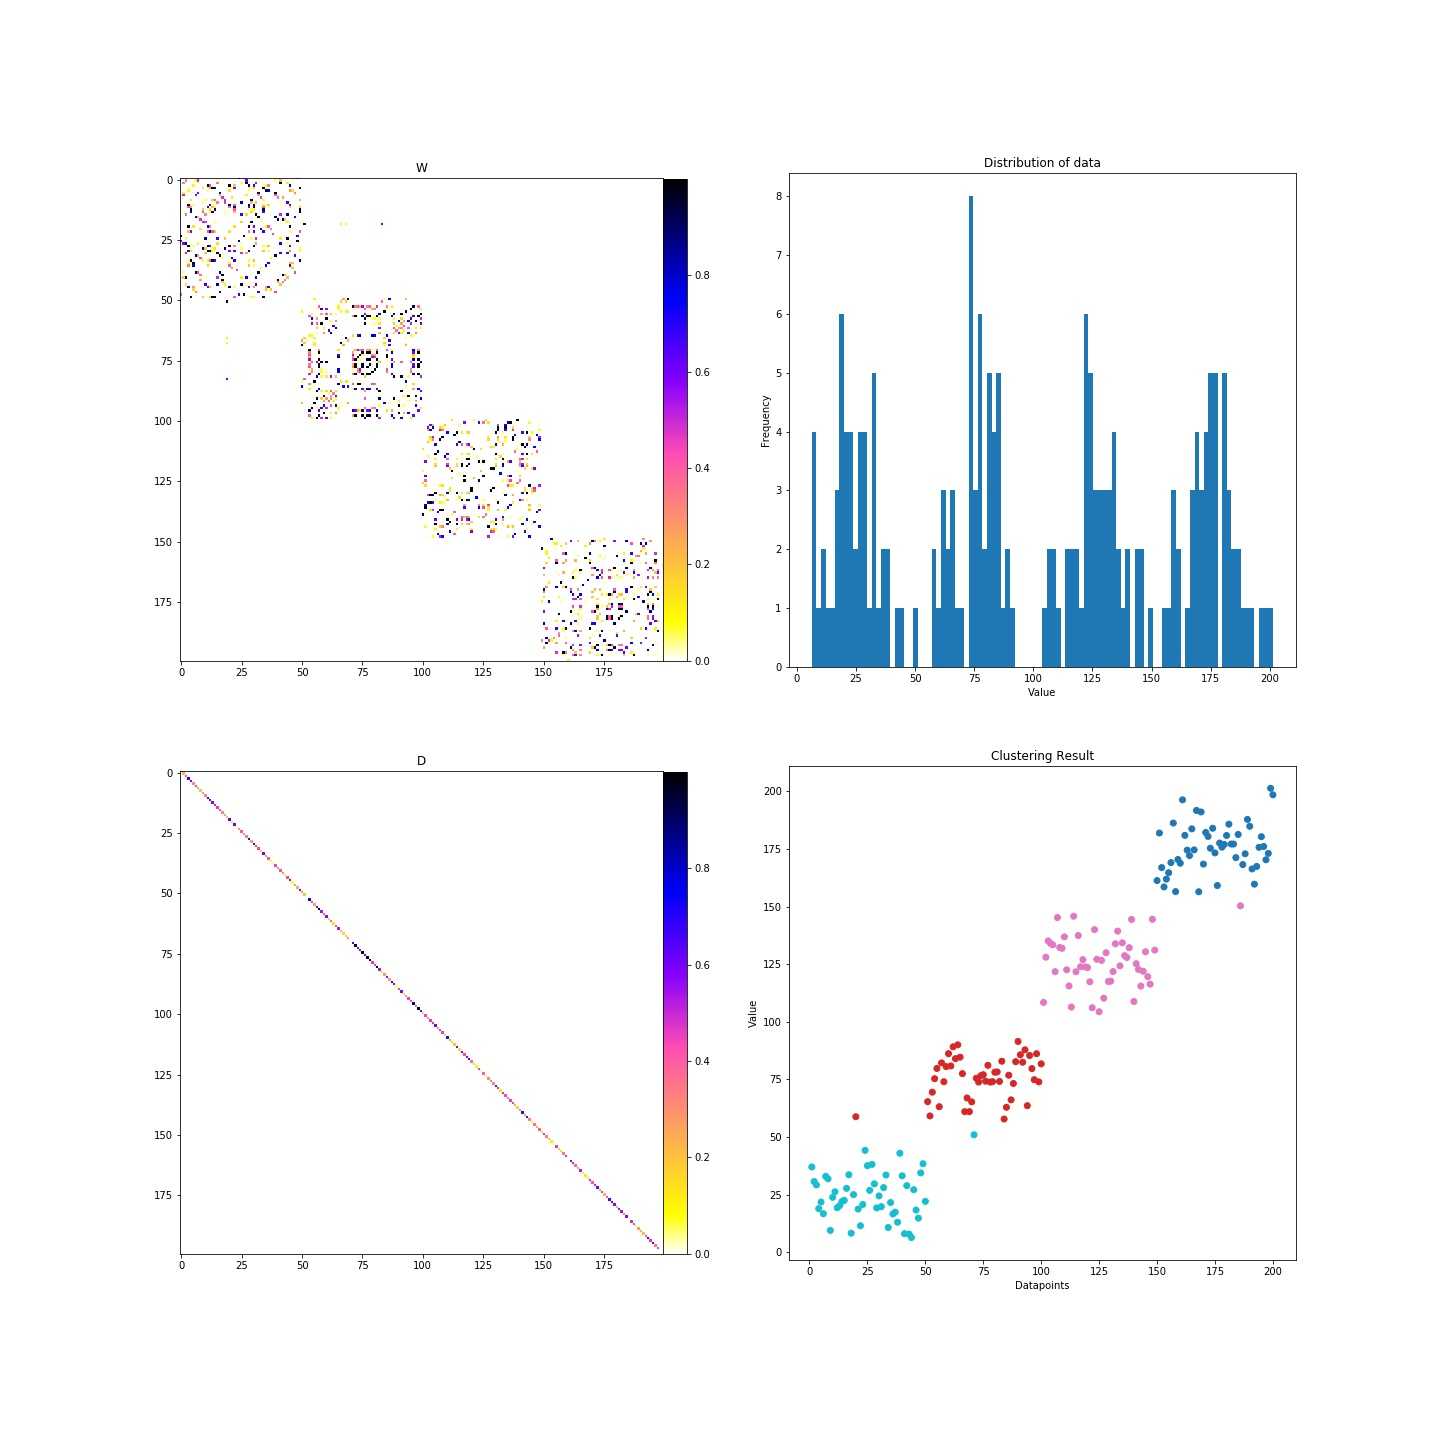
\includegraphics[width=0.9\textwidth]{../../1DCluster.jpg}
        \caption{Clustering results for 200 points in $\mathbb{R}^1$}
        \label{fig:1dresults}
        \end{figure}

        \item{Points in $\mathbb{R}^2$}\\
        This data set consists of 1351 points in $\mathbb{R}^2$ distributed in 9 clusters with one outlier. The figure below shows the clustering in 5, 8 and 10 clusters. This example shows that even though in theory, both Ncut and RatioCut try to keep the clusters reasonably large, that if a single oulier point, if sufficiently separaed from the rest, is clustered independently. The reason for this is that rest of the clusters are very tightly organized. The similarity function used in this case was scaled euclidean distance. The clustering results in to 5, 8 and 10 clusters is shown in Figure \ref{fig:2dresults}

        \begin{figure}
        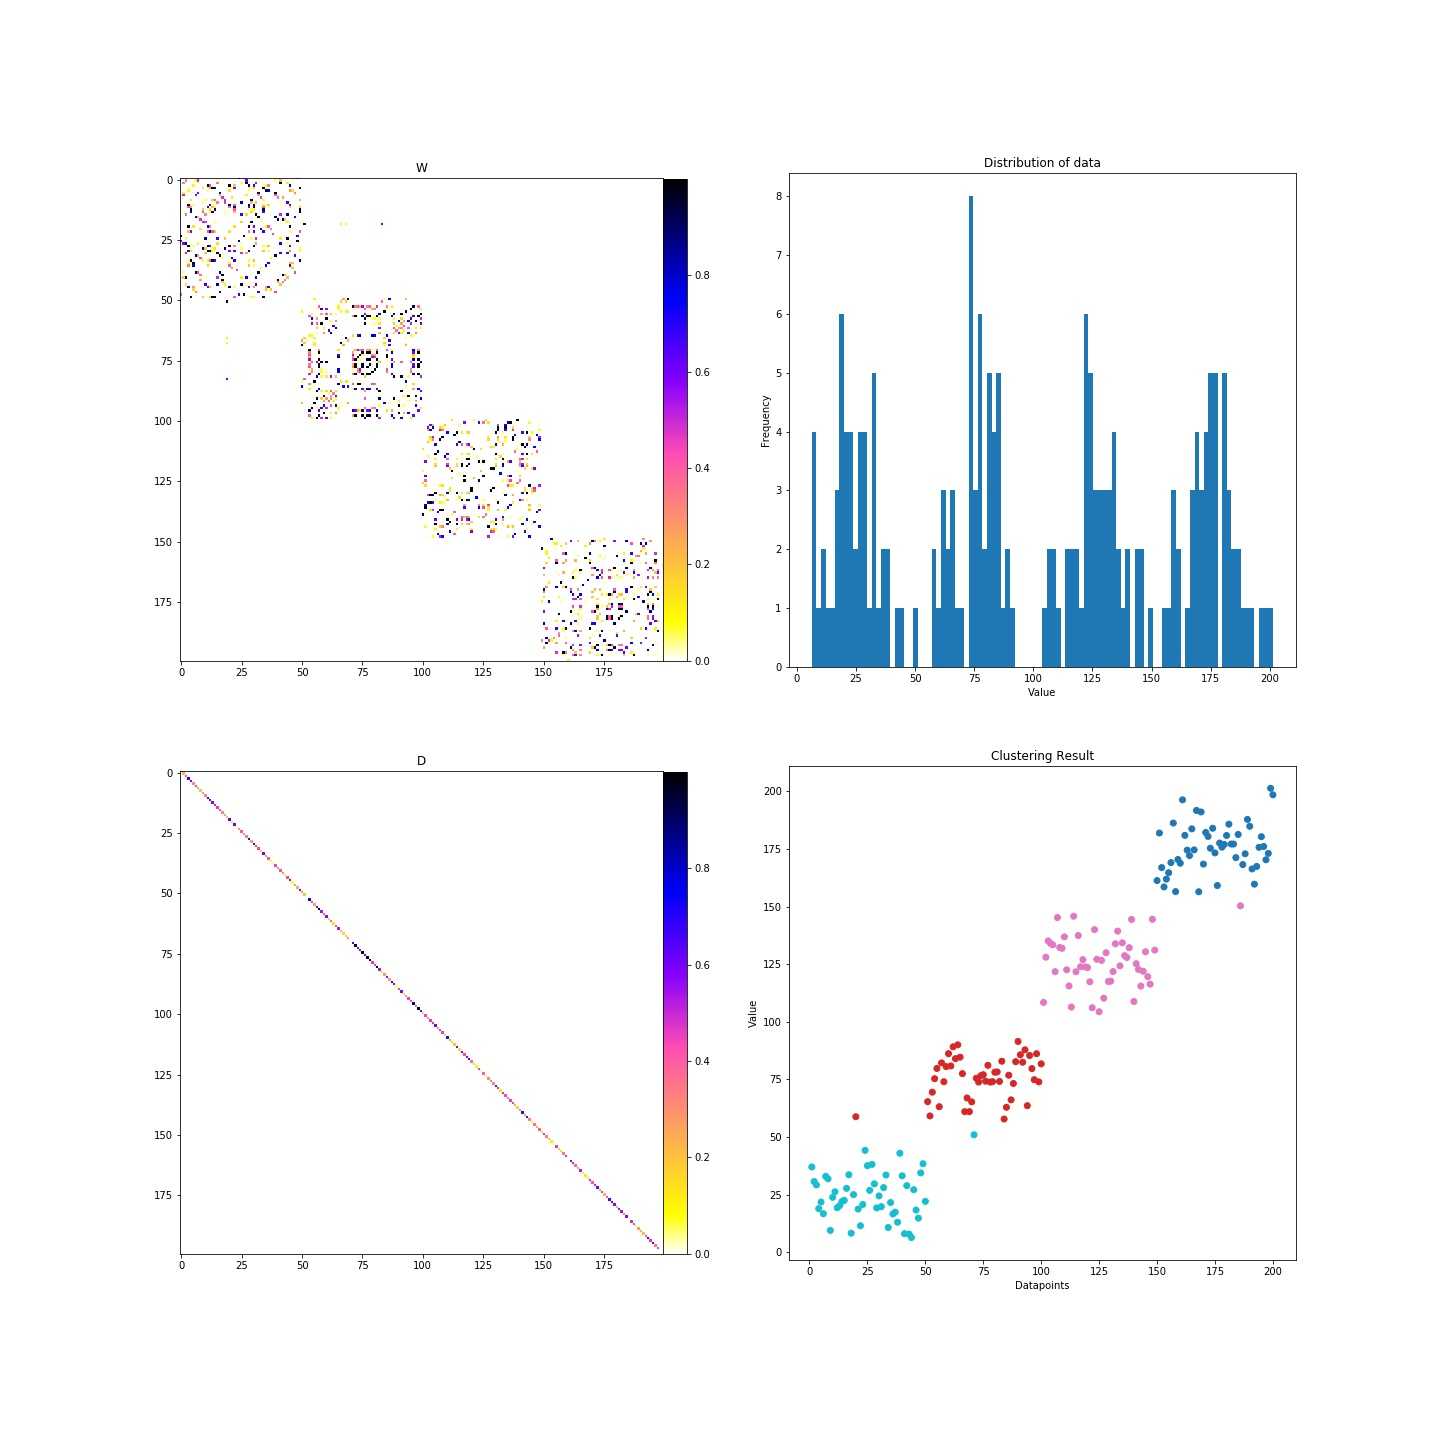
\includegraphics[width=\textwidth]{../../1DCluster.jpg}
        \caption{Clustering results for 200 points in $\mathbb{R}^1$}
        \label{fig:2dresults}
        \end{figure}
    \end{enumerate}
    
    
    \section{Practical considerations and challenges}

    While the algorithms are relatively simple to implement, there are some issues that arise in practice. 
    
    \subsection{Parameters and Tuning Considerations}
    The first consideration is the choice of similarity function. The effectiveness of algorithem depends upon the similarity matrix $W$ which is defined by the similarity function. Although Gaussian similarity function $exp(-\norm{x_I - x_j}^2)/(2\sigma^2)$ is generally a reasonable choice in Euclidean space, the choice of similarity function would generally be guided by the domain of application. 

    Next would be the choice of similarity graph and its parameters. The type of graph ($k$-nearest neighbor, $\epsilon$-neighborhood etc.) affects how the areas of different densities are treated. For example, $k$-nearest neighbor graph may cause some points in a sparse cluster to be connected to a dense cluster or may break a high density cluster into smaller clusters if $k$ is not chosen appropriately. Also for $\epsilon$ neighborhood graph, the choice of $\epsilon$ dicates the sparsity of the matrix. While sparse matrix would be desirable since use of eigensolvers can greatly speedup the eigenvector calculation, it can also lead of loss of information and hence a balance must be achieved and choice of the parameters should be guided by the domain of application. 

    Choice of Laplacian is the next concern. Recall that the goal of clustering is two fold, to minimize inter-cluster similarity or $cut(A,\bar{A})$, and maximize intra-cluster similarity or $W(A,A)$. Both Ncut and RatioCut will achieve the first objective since they both have $cut(A,\bar{A})$ in the numerator. However, note that $W(A,A) = W(A,V) - W(A,\bar{A}) = vol(A) - cut(A,\bar{A})$. This means that intera-cluster similarity is maximized when $cut(A,\bar{A})$ is minimized and $vol(A)$ is maximized. This is where Ncut outperforms RatioCut since it has $vol(A)$ in the denominator. Hence $L_{rw}$ is generally a good choice.

    \subsection{Challanges}

    The following are the challenges that frequently arise in practice. 

    Computing eigenvectors can be an expensive task, particularly if the matrix is large and dense. Fortunately a properly chosen graph and parameter(s) (e.g. $k$ for $k$-means or $\epsilon$ for $\epsilon$ neighborhood), should leads to sparse matrix, which intern facilitates the choice of sparce eigensolvers and hence speed up the calculation. Additionally, the convergence speed depend upon spectral gap $\gamma_k = \abs{\lambda_k - \lambda_{k+1}}$ and convergence depends upon the spectral radius of the matrix. Hence scaling and shifting or even methods like MAPS described in \cite{Lu2015AcceleratedAF} can be applied. 

    Next, challenge would be to choose number of clusters. While the literature that describes the algorithms and their designs, usually takes the number of clusters, $k$, as input to the algorithms, frequently in practice, one needs to find the number of clusters that exist in a dataset. Since this is a general problem for all clustering algorithms, a variety of methods exist. Some methods use the ratio of intra-cluster to inter-cluster similarity or distance as a measure of how good the clustering is, while other methods use statistical calculation based on log-likelihood of data. Additinally, for spectral clustering, eigengap is an important heuristic. A good starting point is to choose $k$ such that $\lambda_1,\dots,\lambda_k$ are small but $\lambda_{k+1}$ is relatively large. However, the effetiveness of this technique depends on how well the clusters are differentiated.

    Finally, the $k$-means step itself can be expensive and in some cases, may not lead to ideal results based on the inital guess and/or the distribution of datapoints. Several attempts have been made to use other techniques of clustering. In \cite{Bottou95convergenceproperties}, the authors show that $k$-means is efficiant and minimizes the quantization error, thus highlight the reasons why $k$-means has become the choice for clustering applications. 
    
    In \cite{tremblay-compressive-SC-16}, the authors propose an algorithm to sample $\mathcal{O}(\log(k))$ randomly fitered signals on the graph to serve as feature vectors instead of eigenvectors and by clustering random subset of $\mathcal{O}(k\log(k))$ nodes using random feature vectors and infering the cluster label of all $N$ nodes. This algorithm speeds up the clustering process by reducing the dimentionality and hence, the size of the problem.

    \section{Optimizations}

    \appendix
    \chapter{Propositions related to Graph Laplacians}
    \begin{prop}(Properties of L) The matrix L satisfies:
        \begin{enumerate}
            \item for every vector $f \in \mathbb{R}^{n}$ we have $$ f_{T}Lf = \frac{1}{2}\sum_{i,j=1}^{n} w_{ij}(f_{i}-f_{j})^{2} $$
            \item L is symmetric and positive semi-definite
            \item The smallest eigenvalue of L is 0, the corresponding eigenvector is the constant vector $\mathbf{1}$
            \item L has $n$ non-negative, real-values eigenvalues $0=\lambda_{1} \le \lambda_{2} \le \cdots \le \lambda_{n}$
        \end{enumerate}
    \end{prop}
    \textit{Proof:}
    \begin{enumerate}
        \item  By definition of $d_{j} = \sum_{i=1}^{n}w_{ij}$
        \begin{align*}
        f'Lf & = f'Df - f'Wf = \sum_{i=1}^{n}d_{i}f_{i}^{2} -  \sum_{i,j=1}^{n}f_{i}f_{j}w_{ij}\\
        & = \frac{1}{2}\bigg(\sum_{i=1}^{n}d_{i}f_{i}^{2} -  2\sum_{i,j=1}^{n}f_{i}f_{j}w_{ij} + \sum_{i=j}^{n}d_{j}f_{j}^{2}\bigg)\\
        & = \frac{1}{2}\sum_{i,j=1}^{n}w_{ij}(f_{i}-f_{j})^{2}
        \end{align*}
        \item Since $W$ and $D$ are symmetric $L = D-W$ is still symmetric. By result of part (a), since $w_{ij} \ge 0$ and $(f_{i}-f_{j})^{2} \ge 0$, $f'Lf \ge 0$, hence $L$ is symmetric and positive semi-definite
        \item See proposition 2
        \item Since $L$ is symmetric, all its eigenvalues are real. Also by part (c), the smallest eigenvalue is 0, 
    \end{enumerate}

    Note that the unnormalized graph Laplacian does not depend on the diagonal elements of $W$. $d_{ii} = \sum_{j=1}^{n}w_{ij}$, hence the diagonal elements are cancelled by $d_{ii}$ and the self-edges do not change the Laplacian. \\
    
    \begin{prop}
        (Number of connected components and the spectrum of $L$) Let $G$ be an undirected graph with non-negative weights. Then the multiplicity $k$ of the engenvalue $0$ of $L$ equals the number of connected components $A_{1},\cdots,A_{k}$ in the graph. The eigenspace of eigenvalue $0$ is spanned by the indicator vectors $\mathbf{1}_{A_{1}},\cdots,\mathbf{1}_{A_{k}}$ of those components.				
    \end{prop}
    \textit{Proof:}
    Starting with $k=1$, i.e. graph is fully connected. Assume that $f$ is the eigenvector with eigenvalue $0$. Then,
    $$ 0 = f'Lf = \sum_{i,j=1}^{n}w_{ij}(f_{i}-f_{j})^{2} \implies f_{i} - f_{j}=0 \hspace{10pt}[\because w_{ij} > 0]$$
    
    Since we assumed a fully connected graph, $f$ has to be constant for the above argument to be true for any vertex in the connected component. Hence the vector $\textbf{1}$, which is the indicator vector of the component is an eigenvector corresponding to eigenvalue $0$. 
    
    Now, for $k>1$, we can easily rearrange the vertices in the matrix to put all the vertices of a connected component together. This would cause the matrix $L$ to be a block diagonal matrix. For each of these blocks, or components, the respective indicator vector is an eigenvector with eigenvalue 0. Thus the Matrix $L$ has eigenvalue $0$ with multiplicity equal to the number of components and the corresponding eigenvectors would be the indicator vectors of those components. 
    $ $\\

    \begin{prop}
        (Properties of $L_{sym}$ and $L_{rw}$)
        \begin{enumerate}
            \item
            For every $f\in\mathbb{R}^{n}$
            $$ f'L_{sym}f = \frac{1}{2}\sum_{i,j=1}^{n}w_{ij}\bigg(\frac{f_{i}}{\sqrt{d_{i}}}-\frac{f_{j}}{\sqrt{d_{j}}}\bigg)^{2} $$
            \item $\lambda$ is an eigenvalue of $L_{rw}$ with eigenvector $u$ iff $\lambda$ is an eigenvalue of $L_{sym}$ with eigenvector $w=D^{1/2}u$.
            \item $\lambda$ is an eigenvalue of $L_{rw}$ with eigenvector $u$ iff $\lambda$ and $u$ solve the generalized eigenproblem $Lu=\lambda Du$
            \item $0$ is an eigenvalue of $L_{rw}$ with the constant one vector $\mathbf{1}$ as eigenvector. $0$ is an eigenvalue of $L_{sym}$ with eigenvector $D^{1/2}\mathbf{1}$
            \item $L_{sym}$ and $L_{rw}$ are positive semi-definite and have $n$ non-negative real-valued eigenvalues $0=\lambda_{1} \le \lambda_{2} \le \cdots \le \lambda_{n}$
        \end{enumerate}
    \end{prop}
    \textit{Proof:}
    \begin{enumerate}
        \item This can be proved similar to part 1 of proposition 1. 
        \item Assume $\lambda$ is an eigenvalue of $L_{sym}$ with eigenvector $w=D^{1/2}u$. 
        \begin{align*}
        L_{sym}D^{1/2}u &= \lambda D^{1/2}u \\
        \implies  D^{-1/2}LD^{-1/2}D^{1/2}u &= \lambda D^{1/2}u \\
        \implies D^{-1}Lu &= \lambda u \hspace{10pt}[\text{left multiplying with } D^{-1/2}] \\
        \implies L_{rw}u &= \lambda u
        \end{align*}
        In otherwords, u is eigenvector of $L_{rw}$. To prove the other direction, apply the above steps in reverse order.
        \item This can be proven in similar manner to above by left multiplying the generalized eigenproblem $Lu = \lambda Du$ with $D^{-1}$
        \item $L_{rw}\mathbf{1} = (I-D^{-1}W)\mathbf{1} = \mathbf{1}-\mathbf{1} = 0$.\\ The above is true because $d_{i} = \sum_{j=1}^{n}wij \implies \big(D^{-1}W)\mathbf{1}\big)_{i} = \sum_{j=1}^{n}\frac{w_{ij}}{d_{i}}$, since $\mathbf{1}$ is the indicator vector. Then using part (b) leads to the second statement of this property. 
        \item The first part (for $L_{sum}$) can be proved from part (a), similar to Proposition 1. Part 2 essentially states that $L_{sym}$ and $L_{rw}$ have the same eigenvalues, hence second statement is also proven.
    \end{enumerate}					

    \begin{prop}
        (Number of connected components and spectra of $L_{sym}$ and $L_{rw}$) Let $G$ be an undirected graph with non-negative weights. Then the multiplicity $k$ of the eigenvalue $0$ of both $L_{sym}$ and $L_{rw}$ equals to the number of connected components $A_{1},\cdots,A_{k}$ in the graph. for $L_{rw}$, the eigenspace of $0$ is spanned by the indicator vectors $\mathbf{1_{A_{i}}}$ of these components. for $L_{sym}$ the eigenspace of $0$ is spanned by $D^{1/2}\mathbf{1_{A_{i}}}$
    \end{prop}
    \textit{Proof:} The proof of this is analogous to that of proposition 2, but using proposition 3.


	\nocite{govl:96, parlet:98,stsu:90,gene:2018}
	
	\thispagestyle{fancy}
	\bibliographystyle{unsrt}
	\bibliography{long_string, Mybib} 
	
\end{document}